\documentclass[english, 12pt, aspectratio=169]{beamer}
\usepackage{amsmath,amssymb,amsthm,amsfonts}
\usepackage{array}
\usepackage[round]{natbib}
\renewcommand{\bibsection}{}
\usepackage{url}
% \usepackage{fontawesome}
\usepackage{graphicx}
\usepackage{booktabs}
\usepackage{multirow}
\usepackage{doi}
\usepackage[export]{adjustbox} % for framed includegraphics
\usetheme{metropolis}
\usepackage[default]{sourcesanspro}
\usepackage{tcolorbox}
\usepackage{fontawesome} % fontawesome icons
\usepackage{tikz}
\usepackage{svg}
\usepackage{pdfpages}
\usetikzlibrary{positioning, arrows, fadings,decorations.pathmorphing,arrows.meta, shapes.arrows}
\tikzset{
  % Define standard arrow tip
  >=stealth',
  % Define style for boxes
  punkt/.style={
    rectangle,
    rounded corners,
    draw=black, very thick,
    text width=6.5em,
    minimum height=10em,
    minimum width = 10em
    text centered},
  % Define arrow style
  pil/.style={
    ->,
    thick,
    shorten <=2pt,
    shorten >=2pt,}
}

%% colors
\definecolor{nicegreen}{HTML}{008000}
\definecolor{niceblue}{RGB}{30, 126, 229}
\definecolor{nicered}{RGB}{216, 27, 96}
\definecolor{lightlightgray}{RGB}{211,211,211} % for tikz diagram
%\definecolor{lightred}{RGB}{249,174,174} % for tikz diagram
%\definecolor{lightred}{RGB}{255, 204, 118} % for tikz diagram
\definecolor{lightred}{RGB}{253, 169, 104} % for tikz diagram
\definecolor{dark2green}{RGB}{27, 158, 119}
\definecolor{dark2purple}{RGB}{117, 112, 179}
\definecolor{dark2orange}{RGB}{217, 95, 2}
\definecolor{chineseBlue}{RGB}{60, 88, 152}
\definecolor{metallicBlue}{RGB}{41, 72, 125}
\definecolor{wildBlueYonder}{RGB}{156, 178, 206}
\definecolor{gainsboro}{RGB}{212, 216, 232}
\setbeamercolor{frametitle}{bg = metallicBlue}
\setbeamercolor{progress bar}{fg = metallicBlue}
\setbeamercolor{alerted text}{fg=dark2orange}

% red from R ; % blue from R ; % green from R Set 1
\definecolor{Rred}{RGB}{228, 26, 28}
\definecolor{Rgreen}{RGB}{77, 175, 74}
\definecolor{Rblue}{RGB}{55, 126, 184}

\usepackage{hyperref}
\hypersetup{
  pdftitle={Simulation Studies for Methodological Research in Psychology},
  pdfsubject={Björn Siepe}
}



\date{$\star$ Psychological Methods Lab, Department of Psychology, University of Marburg}
\title{~\\ ~ \\ \textbf{Simulation Studies for Methodological Research in Psychology}}
\author{\textbf{Björn S. Siepe}\textsuperscript{$\star$}, František Bartos, Tim P. Morris, Anne-Laure Boulesteix, Daniel Heck, Samuel Pawel}
\institute{
  DagStat2025. Slides available at \url{htpps://bsiepe.github.io}
}
\titlegraphic{
  \includegraphics[width = 0.2\textwidth]{pics/UMR-logo.png}
}

% TODOS
% slide 9: doesn't need to be as extensive
% template: make example/explanation text more visually distinct
% add qr code
% slide 7: maybe just show upper row first
% slide 5: boxes for parameters, metrics,... could be in a light grey


\usepackage{Sweave}
\begin{document}
\Sconcordance{concordance:DagStat25-Bjoern-Siepe.tex:DagStat25-Bjoern-Siepe.Rnw:1 90 %
1 1 0 570 1}



\begin{frame}[noframenumbering, plain]
  \titlepage
\nocite{PawelKookReeve2023}
\end{frame}


\begin{frame}{Simulation studies}
  \centering
  \pause
  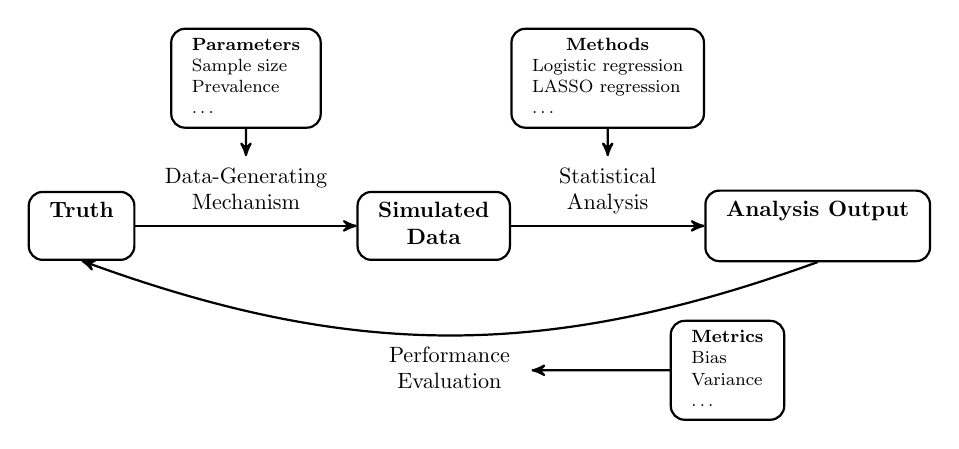
\begin{tikzpicture}[thick,scale=0.8, every node/.style={scale=0.8}]

    % nodes
    \node [rectangle, draw, rounded corners = 0.5em] (truth)
    {\begin{tabular}{c} \textbf{Truth} \\
       \phantom{$\theta$}
     \end{tabular}};

   % \uncover<2->{
   \node [rectangle, draw, rounded corners = 0.5em] (simdat) [right = 8em of truth]
   {\begin{tabular}{c} \textbf{Simulated} \\
      \textbf{Data}
    \end{tabular}};
  %}

  % \uncover<3->{
  \node [rectangle, draw, rounded corners = 0.5em] (output) [right = 7em of simdat]
  {\begin{tabular}{c} \textbf{Analysis Output} \\
     \phantom{$\hat{\theta}$}
   \end{tabular}};
 %}


 % edges
 \draw [->] (truth) -- node [above] (dgp)
 {  \begin{tabular}{c} Data-Generating \\ Mechanism \end{tabular}}
 (simdat);

 \draw [->] (simdat) -- node [above] (analysis)
 {  \begin{tabular}{c} Statistical \\ Analysis \end{tabular}}
 (output);

 \draw [->] (output.south) to [bend left = 20]  node [below, sloped] (performance)
 {   \begin{tabular}{c} Performance \\ Evaluation \end{tabular}}
 (truth.south);

  % nodes related to edges
 \node [rectangle, draw, rounded corners = 0.5em] (methods) [above = 1em of analysis]
 {\footnotesize \begin{tabular}{l}
                  \multicolumn{1}{c}{\textbf{Methods}} \\
           Logistic regression \\ LASSO regression \\ $\hdots$  \end{tabular}};

  \node [rectangle, draw, rounded corners = 0.5em] (params) [above = 1em of dgp]
       {\footnotesize \begin{tabular}{l} \textbf{Parameters} \\
                 Sample size \\ Prevalence \\ $\hdots$  \end{tabular}};

  \node [rectangle, draw, rounded corners = 0.5em] (metrics) [right = 5em of performance]
       {\footnotesize \begin{tabular}{l} \textbf{Metrics} \\
                 Bias \\ Variance \\ $\hdots$  \end{tabular}};

   \draw [->] (params.south) to (dgp);
  \draw [->] (methods.south) to (analysis);
  \draw [->] (metrics.west) to (performance.east);
\end{tikzpicture}
\end{frame}

\begin{frame}{Simulation studies can have huge impact}

  % \begin{block}{}
  %   \begin{tcolorbox}[colframe=chineseBlue]
  %     \centering
  %       \large Simulation studies can have \alert{\textbf{huge impact}}
  %     \end{tcolorbox}
  % \end{block}


    \begin{block}{}
          \begin{columns}
      \begin{column}{0.5\textwidth}
        \centering
        
\includegraphics[width=1.05\textwidth,frame]{pics/peduzzi.png}
      \end{column}
      \begin{column}{0.5\textwidth}
        \centering
        
\includegraphics[width=1.05\textwidth,frame]{pics/hubentler.png}

      \end{column}
      \end{columns}
    \end{block}

      \begin{block}{}
          \begin{columns}
      \begin{column}{0.5\textwidth}
        \centering
        
\includegraphics[width=1.05\textwidth,frame]{pics/dormann.png}
      \end{column}
      \begin{column}{0.5\textwidth}
        \centering
        
\includegraphics[width=1.05\textwidth,frame]{pics/nylund.png}

      \end{column}
      \end{columns}
    \end{block}



\end{frame}




\begin{frame}{Issues in simulation studies}
    \begin{block}{}
      \begin{tcolorbox}[colframe=chineseBlue]
        ``\emph{\dots extensive simulation studies show that the proposed
          method performs on par or \textbf{\alert{better than existing
              methods}} \dots}''
      \end{tcolorbox}

    \end{block}
    
    \begin{block}{}
      \begin{columns}
      \begin{column}{0.5\textwidth}
      \pause
        \begin{itemize}
          \item Over-Optimism \citep[e.g.,][]{Ullmann2022}
          \pause
          \item Insufficient reporting standards \citep[e.g.,][]{Hoaglin1975}
          \pause
          \item Little assessment of reproducibility \citep[e.g.,][]{Luijken2023}
        \end{itemize}
      \end{column}
      \begin{column}{0.5\textwidth}
      \pause
        \centering
        
\includegraphics[width=0.35\textwidth]{pics/questionXKCD.png}

        {\tiny \color{gray} \href{https://xkcd.com}{xkcd.com} (CC-BY-NC)}
      \end{column}
      \end{columns}
    \end{block}
  \end{frame}
\begin{frame}{Issues in simulation studies}
    \begin{columns}
      \begin{column}{0.65\textwidth}
        \begin{block}{}
          \begin{tcolorbox}[colframe=chineseBlue]
            ``\emph{In fact it is \alert{\textbf{very difficult to run an \mbox{honest} simulation}} comparison, and \alert{\textbf{easy to \mbox{inadvertently} cheat}} by choosing favorable examples, or by not putting as much effort into optimizing the dull old standard as the exciting new challenger.}''

            \flushright Brad Efron (\citeyear{Breiman2001}) % [p.219]\\''
          \end{tcolorbox}
        \end{block}
      \end{column}
      \begin{column}{0.35\textwidth}
        \begin{block}{}
          \centering
          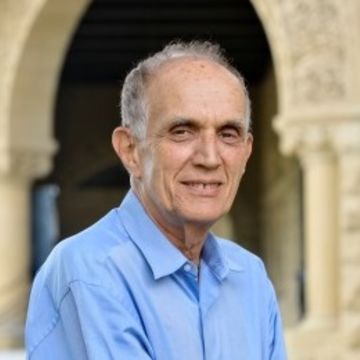
\includegraphics[width=0.8\linewidth,frame]{pics/efron2.jpg}
          {\tiny \color{gray} \href{https://statistics.stanford.edu/people/bradley-efron}{https://statistics.stanford.edu/people/bradley-efron}}
        \end{block}
      \end{column}
    \end{columns}
    
\end{frame}


\begin{frame}{Questionable research practices in simulation studies}
  \centering
  \only<1,2>{
  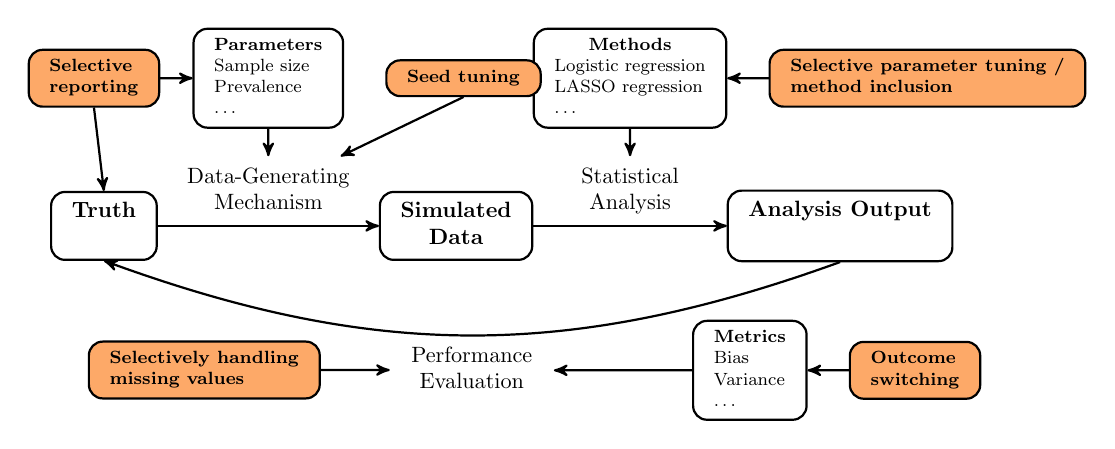
\begin{tikzpicture}[thick,scale=0.8, every node/.style={scale=0.8}]

    % nodes
    \node [rectangle, draw, rounded corners = 0.5em] (truth)
    {\begin{tabular}{c} \textbf{Truth} \\
       \phantom{$\theta$}
     \end{tabular}};

   % \uncover<2->{
   \node [rectangle, draw, rounded corners = 0.5em] (simdat) [right = 8em of truth]
   {\begin{tabular}{c} \textbf{Simulated} \\
      \textbf{Data}
    \end{tabular}};
  %}

  % \uncover<3->{
  \node [rectangle, draw, rounded corners = 0.5em] (output) [right = 7em of simdat]
  {\begin{tabular}{c} \textbf{Analysis Output} \\
     \phantom{$\hat{\theta}$}
   \end{tabular}};
 %}


 % edges
 \draw [->] (truth) -- node [above] (dgp)
 {  \begin{tabular}{c} Data-Generating \\ Mechanism \end{tabular}}
 (simdat);

 \draw [->] (simdat) -- node [above] (analysis)
 {  \begin{tabular}{c} Statistical \\ Analysis \end{tabular}}
 (output);

 \draw [->] (output.south) to [bend left = 20]  node [below, sloped] (performance)
 {   \begin{tabular}{c} Performance \\ Evaluation \end{tabular}}
 (truth.south);

  % nodes related to edges
 \node [rectangle, draw, rounded corners = 0.5em] (methods) [above = 1em of analysis]
 {\footnotesize \begin{tabular}{l}  \multicolumn{1}{c}{\textbf{Methods}} \\
           Logistic regression \\ LASSO regression \\ $\hdots$  \end{tabular}};

  \node [rectangle, draw, rounded corners = 0.5em] (params) [above = 1em of dgp]
       {\footnotesize \begin{tabular}{l} \textbf{Parameters} \\
                 Sample size \\ Prevalence \\ $\hdots$  \end{tabular}};

  \node [rectangle, draw, rounded corners = 0.5em] (metrics) [right = 5em of performance]
       {\footnotesize \begin{tabular}{l} \textbf{Metrics} \\
                 Bias \\ Variance \\ $\hdots$  \end{tabular}};

   % QRP nodes
   \uncover<2>{\node [rectangle, draw, rounded corners = 0.5em, fill = lightred] (tuning) [right = 1.5em of methods]
       {\footnotesize \begin{tabular}{l}
       {\textbf{Selective parameter tuning /}} \\
       {\textbf{method inclusion}}
       \end{tabular}};

    \node [rectangle, draw, rounded corners = 0.5em, fill = lightred] (switching) [right = 1.5em of metrics]
       {\footnotesize \begin{tabular}{l}
       {\textbf{Outcome}} \\
       {\textbf{switching}}
       \end{tabular}};

    \node [rectangle, draw, rounded corners = 0.5em, fill = lightred] (selectreport) [left = 1.18em of params]
       {\footnotesize \begin{tabular}{l}
       {\textbf{Selective}} \\
       {\textbf{reporting}}
       \end{tabular}};

    \node [rectangle, draw, rounded corners = 0.5em, fill = lightred] (seed) [right = 1.5em of params]
       {\footnotesize \begin{tabular}{l}
       {\textbf{Seed tuning}}
       \end{tabular}};

    \node [rectangle, draw, rounded corners = 0.5em, fill = lightred] (inclusion) [left = 2.5em of performance]
       {\footnotesize \begin{tabular}{l}
       {\textbf{Selectively handling}} \\
       {\textbf{missing values}}
                      \end{tabular}};
}

  \draw [->] (params.south) to (dgp);
  \draw [->] (methods.south) to (analysis);
  \draw [->] (metrics.west) to (performance.east);
\uncover<2>{
  \draw [->] (tuning.west) to (methods.east);
  \draw [->] (switching.west) to (metrics.east);
  \draw [->] (selectreport.east) to (params.west);
  \draw [->] (selectreport.south) to (truth.north);
  \draw [->] (seed.south) to (dgp);
  % \draw [->] (seed.east) to (methods.west);
  \draw [->] (inclusion.east) to (performance.west);
}
\end{tikzpicture}
}
\only<3>{

  \begin{block}{}
    \centering
    
\includegraphics[width = 0.8\linewidth,frame]{pics/biometr2023.png}

    \vspace{0.5em}

    \begin{tcolorbox}[colframe=chineseBlue]
      ``\emph{By \alert{\textbf{deliberately using several QRPs}}, we were able
        to \alert{\textbf{present a method with no expected benefits}} [\dots]
        \alert{\textbf{as an improvement}} over [\dots] well-established
        competitors.}''
    \end{tcolorbox}
    \end{block}

    \nocite{PawelKookReeve2023}
    % \vfill
    % \flushleft {\tiny \color{gray} \href{https://doi.org/10.1002/bimj.202200091}{doi.org/10.1002/bimj.202200091}}

  }

\end{frame}

% \begin{frame}{Questionable research practices in simulation studies}
%   \begin{columns}
%     \begin{column}{0.8\textwidth}
%       \begin{block}{Root causes}
%         \begin{itemize}
%           \item \alert{{Pressure to publish}} novel and positive results
%           \item \alert{{Low requirements}} from journals
%           \item \alert{{Cognitive biases}} (e.g., confirmation or hindsight
%                 bias)
%           \item \alert{{Low awareness}} in scientific community
%         \end{itemize}
%       \end{block}
%       \uncover<3>{
%         \begin{block}{Potential consequences}
%           \begin{itemize}
%             \item \alert{{Overoptimistic conclusions}}
%             \item \alert{{Publication bias}}
%             \item \alert{{Misinformed decisions}}
%           \end{itemize}
%         \end{block}
%       }
%     \end{column}
%     \begin{column}{0.2\textwidth}
%       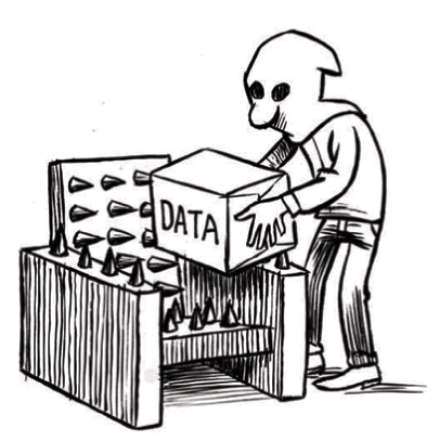
\includegraphics[width=\textwidth]{pics/datatorture.png}

%       \vspace{1em}

%       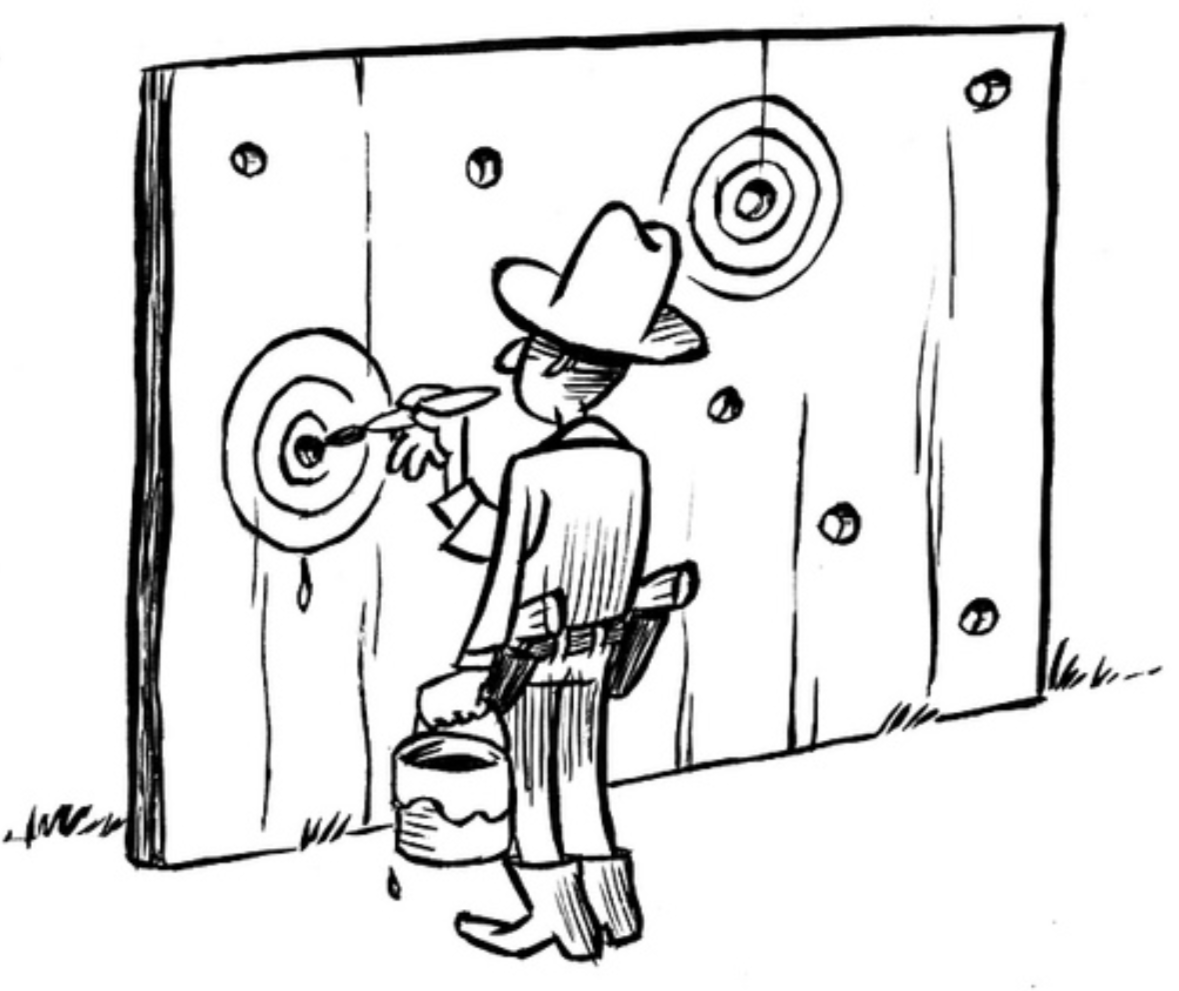
\includegraphics[width = 1\textwidth]{pics/TexasSharpShooter.png}

%       {\tiny \color{gray} Dirk-Jan Hoek (CC-BY)}

%     \end{column}
%   \end{columns}
% \end{frame}

%\begin{frame}{Replicability of simulation studies}

%  \vspace{-2em}
%  \begin{block}{}
%    \begin{figure}
%      \centering
%      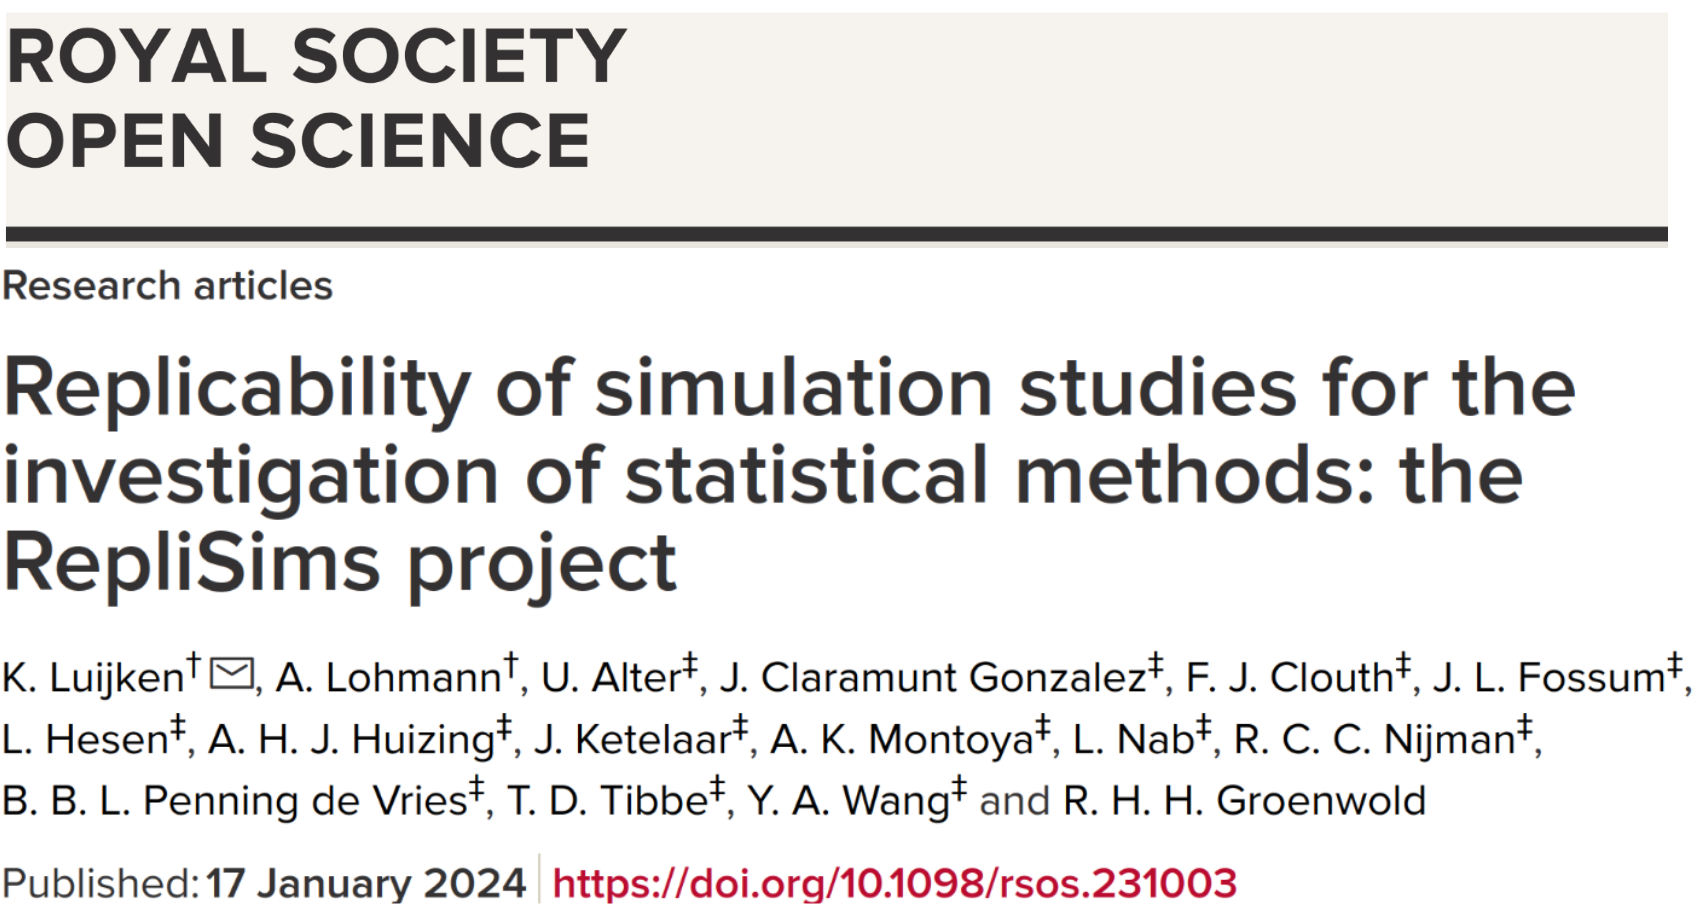
\includegraphics[width = 0.6\textwidth,frame]{pics/luijken2024.png}
%    \end{figure}
%
%    \begin{tcolorbox}[colframe=chineseBlue]
%      ``\emph{the information provided in the original publication of highly cited
%        and influential simulation studies was \textbf{\alert{often insufficient
%            for complete replication}}}''
%    \end{tcolorbox}
%
%    {\tiny \color{gray} \citet{Luijken2023}, \href{https://doi.org/10.48550/ARXIV.2307.02052}{doi.org/10.48550/ARXIV.2307.02052}}
%  \end{block}
% \end{frame}

\begin{frame}{Literature Review}
\begin{tcolorbox}[colframe=chineseBlue]
            ``\emph{Statisticians ... often pay too little attention to their own principles of design}''(Hoaglin \& Andrews, 1975)
          \end{tcolorbox}
          \vspace{-1em}
  \begin{columns}
    \begin{column}{0.5\textwidth}
      \begin{block}{}
          \centering
          
\includegraphics[width = 0.8\linewidth,frame]{pics/hoaglin.png}
          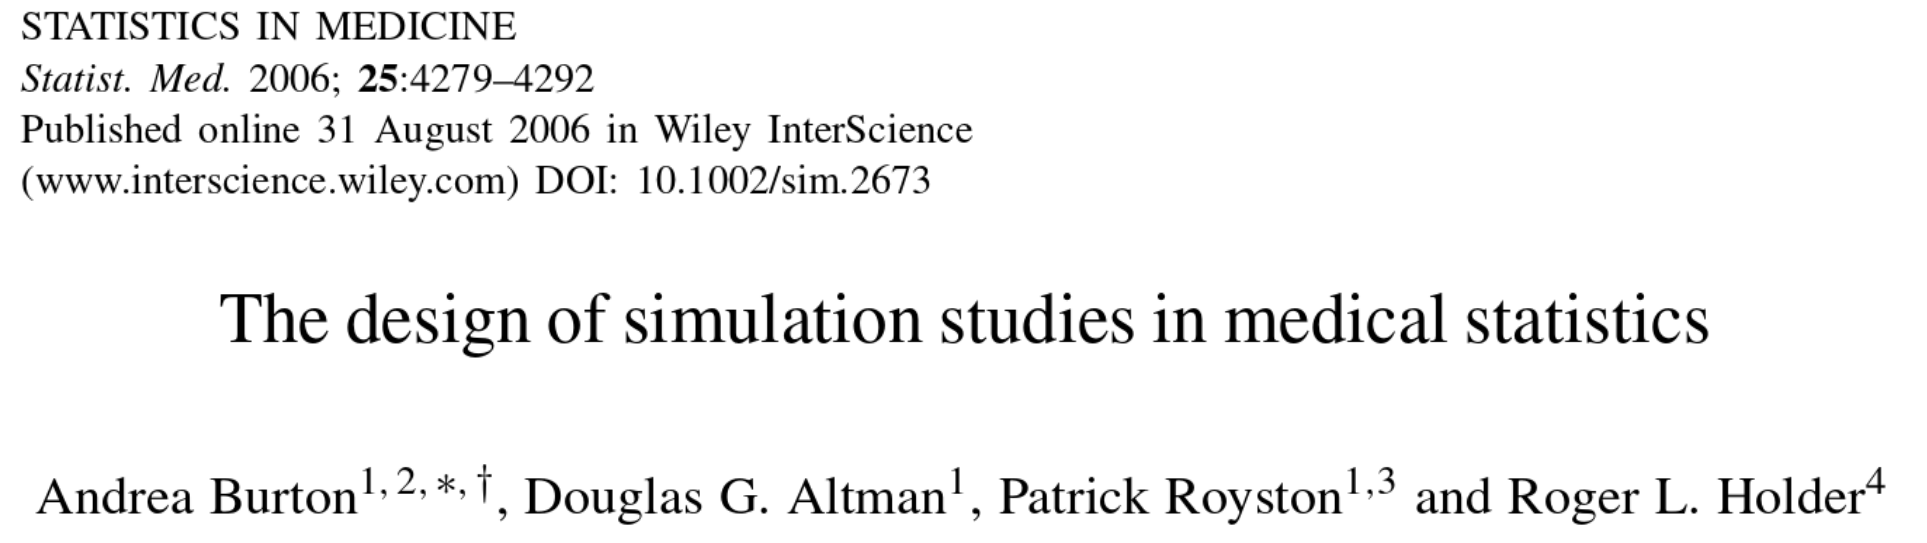
\includegraphics[width = 0.8\linewidth,frame]{pics/burton.png}
          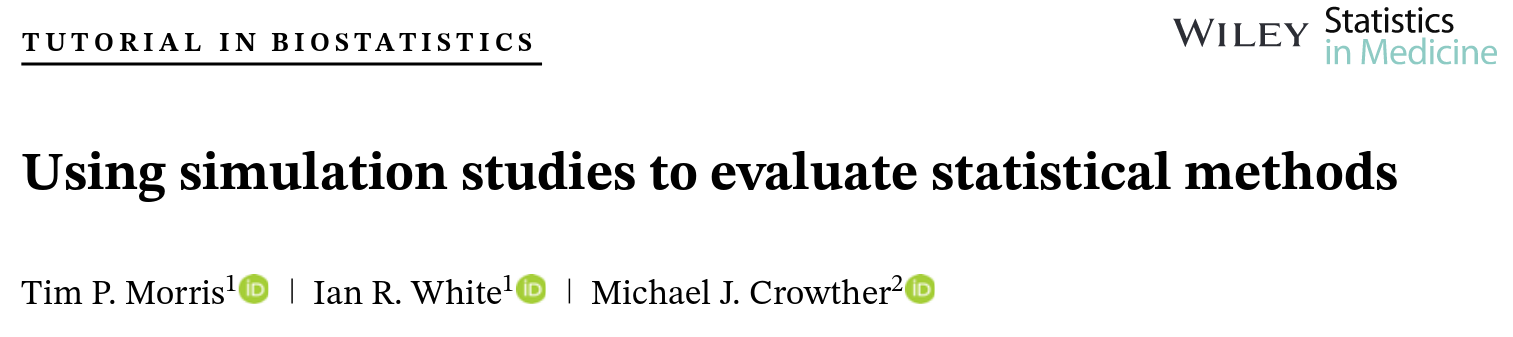
\includegraphics[width = 0.8\linewidth,frame]{pics/morris.png}
          \nocite{Hoaglin1975}
          \pause
      \end{block}
    \end{column}
    \begin{column}{0.5\textwidth}
      \begin{block}{}
      \textbf{This project:}
      \pause
        \begin{itemize}
          \item Review of \alert{100 recent simulation studies} in psychology
          \pause
          \item Psychological Methods, Behavior Research Methods, Multivariate Behavioral Research
          \pause
          \item Coding of various aspects of reporting
        \end{itemize}
      \end{block}
      \end{column}
    \end{columns}
\end{frame}


\begin{frame}{Main Results}
\pause
   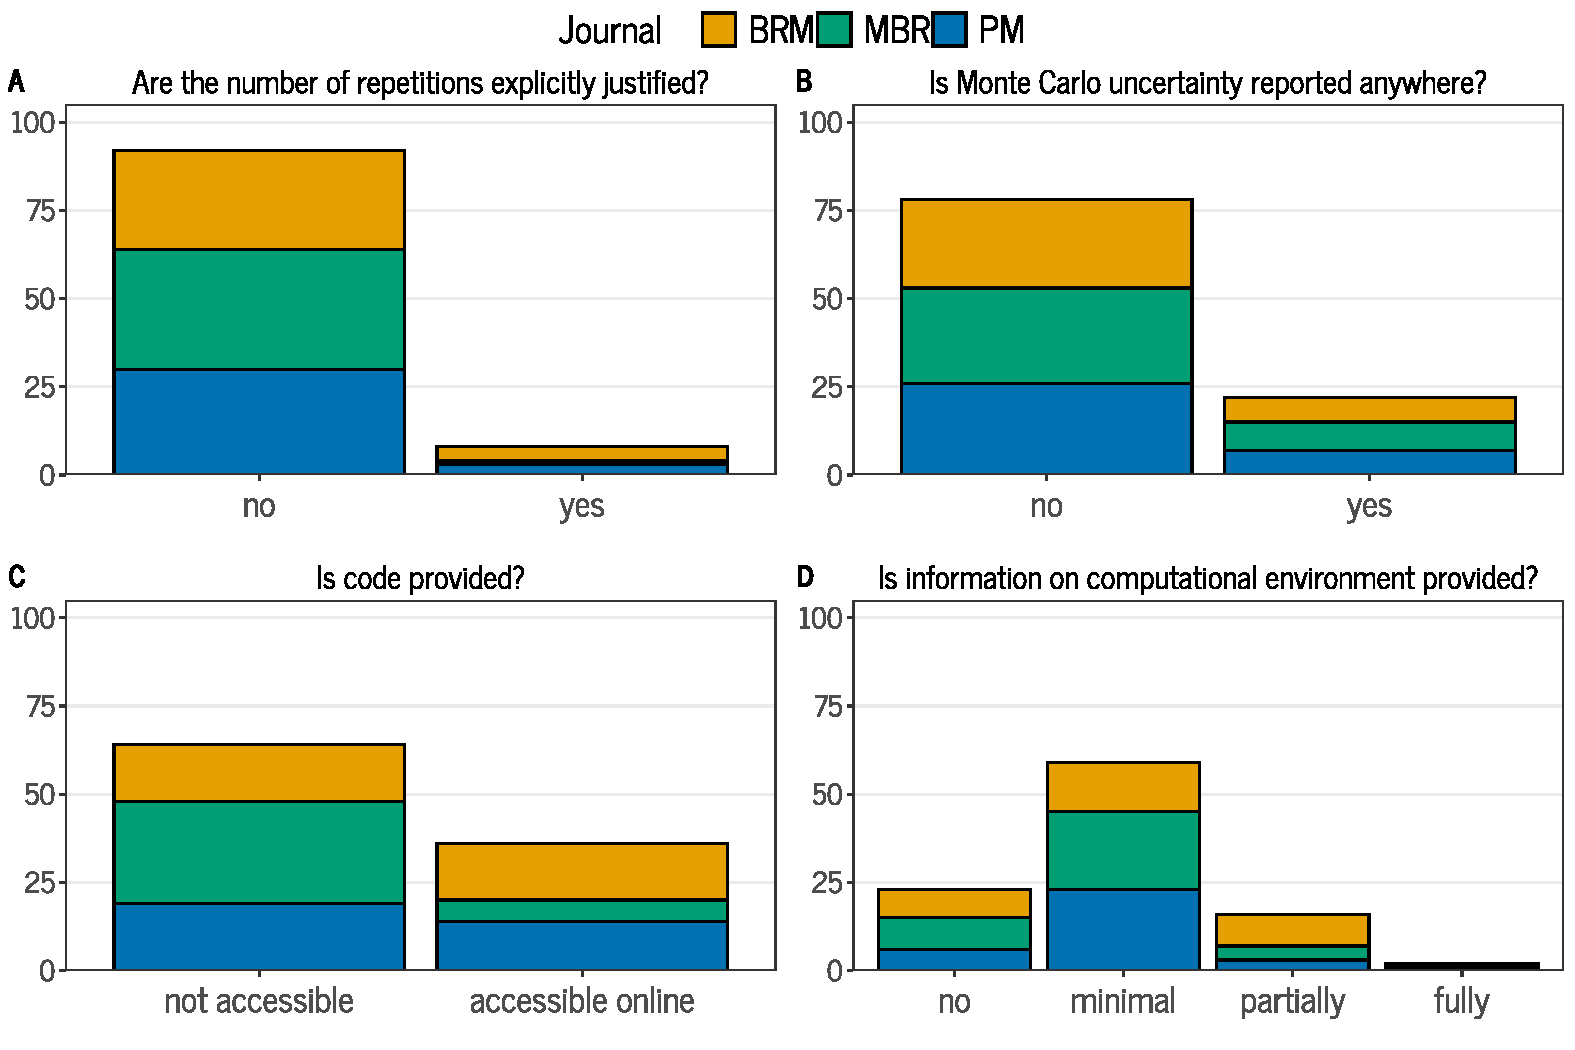
\includegraphics{pics/review-results.pdf}
\end{frame}


% \begin{frame}{Simulation study protocols}
%   \begin{block}{}
%     \centering
%     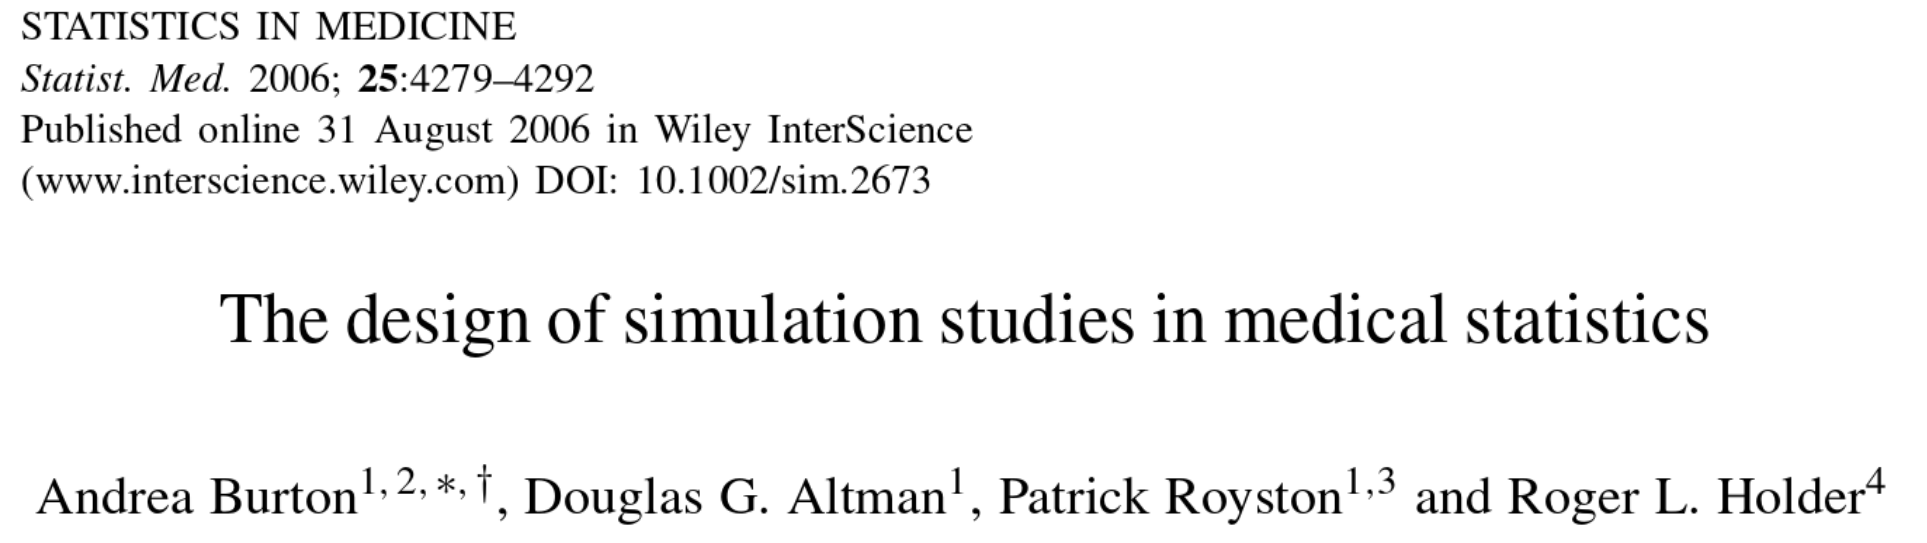
\includegraphics[width = 0.8\linewidth,frame]{pics/burton.png}
%     \nocite{Burton2006}
% 
%   \end{block}
%   \begin{block}{}
%     \begin{tcolorbox}[colframe=chineseBlue]
%       ``\emph{\alert{\textbf{When planning}} a simulation study, it is
%         \alert{\textbf{recommended that a detailed protocol be produced}},
%         giving full details of how the study will be performed, analysed and
%         reported.}''
%     \end{tcolorbox}
%   \end{block}
% 
%   \vfill
%   % \flushleft {\tiny \color{gray} \href{https://doi.org/10.1002/sim.2673}{doi.org/10.1002/sim.2673}}
% 
% \end{frame}

% \begin{frame}{Simulation study protocols}
%   \begin{columns}
%     \begin{column}{0.5\textwidth}
%       \begin{block}{Advantages}
%         \begin{itemize}
%         \pause
%           \item[+] Planning and reporting
%           \pause
%           \item[+] Transparency and replicability
%           \pause
%           \item[+] Can be preregistered
%           \pause
%           \item[?] Less/more work
%         \end{itemize}
%       \end{block}
% 
%       \begin{block}{}
%         \begin{itemize}
%           \item[$\rightarrow$] \alert{\textbf{How to structure protocol?}}
%         \end{itemize}
%       \end{block}
% 
%     \end{column}
%     \begin{column}{0.5\textwidth}
%       \begin{block}{}
%       \centering
%       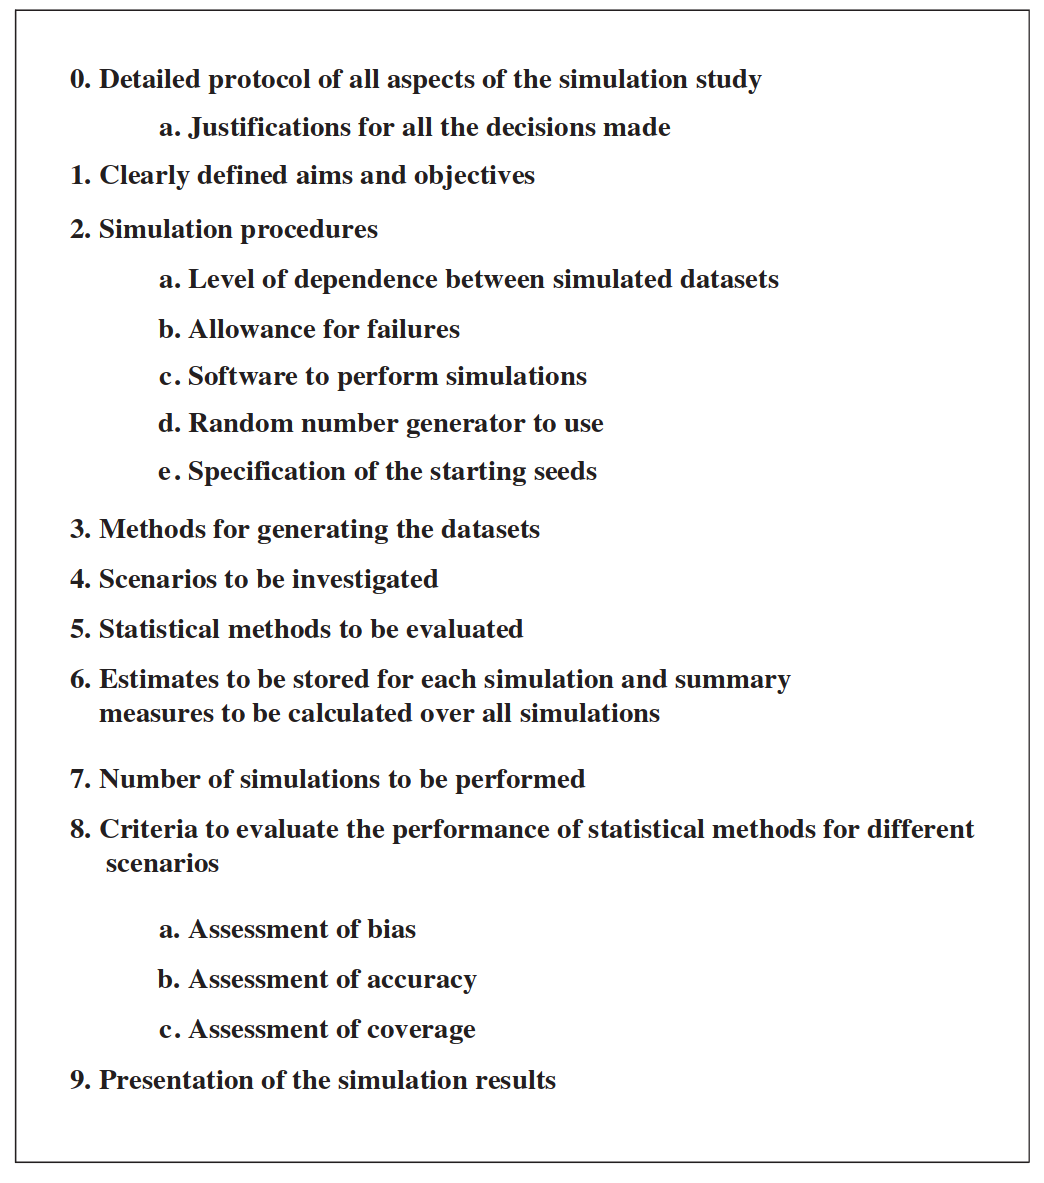
\includegraphics[width=0.7\textwidth]{pics/burtonprotocol.png} \\
%       Proposal from \citet{Burton2006}
%       \end{block}
%     \end{column}
%   \end{columns}
% 
%  \end{frame}

\begin{frame}{Towards improved reporting}
  \begin{block}{}
  \centering
  
\includegraphics[width = 0.6\linewidth,frame]{pics/ademprereg.png}

  \begin{itemize}
  \pause
    \item Protocol template based on \alert{\textbf{ADEMP structure}}
          \citep{Morris2019} + \alert{\textbf{open~science}} +
          \alert{\textbf{reproducibility}} aspects
    % \item Purposes: \alert{preregistration}, \alert{reporting/planning/reviewing
    %       blueprint}
    \pause
    \item \alert{\textbf{Different versions}}: \LaTeX, Overleaf, MS/Libre office, Google
    docs
    \pause
    \item \alert{\textbf{Living
          document}}:          \href{https://github.com/bsiepe/ADEMP-PreReg}{https://github.com/bsiepe/ADEMP-PreReg}
    \end{itemize}
  \end{block}

  \vspace{-1.5em}
  \nocite{Siepe2023}
  \flushleft {\tiny \color{gray}
    \href{https://doi.org/10.1214/ss/1009213726}{ADEMP: doi.org/10.1214/ss/1009213726},
    \href{https://doi.org/10.31234/osf.io/ufgy6}{ADEMP-PreReg: doi.org/10.31234/osf.io/ufgy6}
    }
 % \href{https://www.overleaf.com/latex/templates/ademp-prereg-simulation-study-template/dkhtxjtmpbfj}{overleaf.com/latex/templates/ademp-prereg-simulation-study-template/dkhtxjtmpbfj}}

\end{frame}

\begin{frame}{The ADEMP-PreReg template}
  \begin{columns}
    \begin{column}{0.5\textwidth}
  \begin{block}{}
    \begin{enumerate}
    \item Instructions
    \item General information
    \item \alert{\textbf{A}}ims
    \item \alert{\textbf{D}}ata-generating mechanism
    \item \alert{\textbf{E}}stimands and targets
    \item \alert{\textbf{M}}ethods
    \item \alert{\textbf{P}}erformance Measures
    \item Computational details
    \pause
    \end{enumerate}
    \nocite{Burton2006}
  \end{block}
\end{column}
\begin{column}{0.5\textwidth}
  \centering
  \vspace{1em}

    % \only<1>{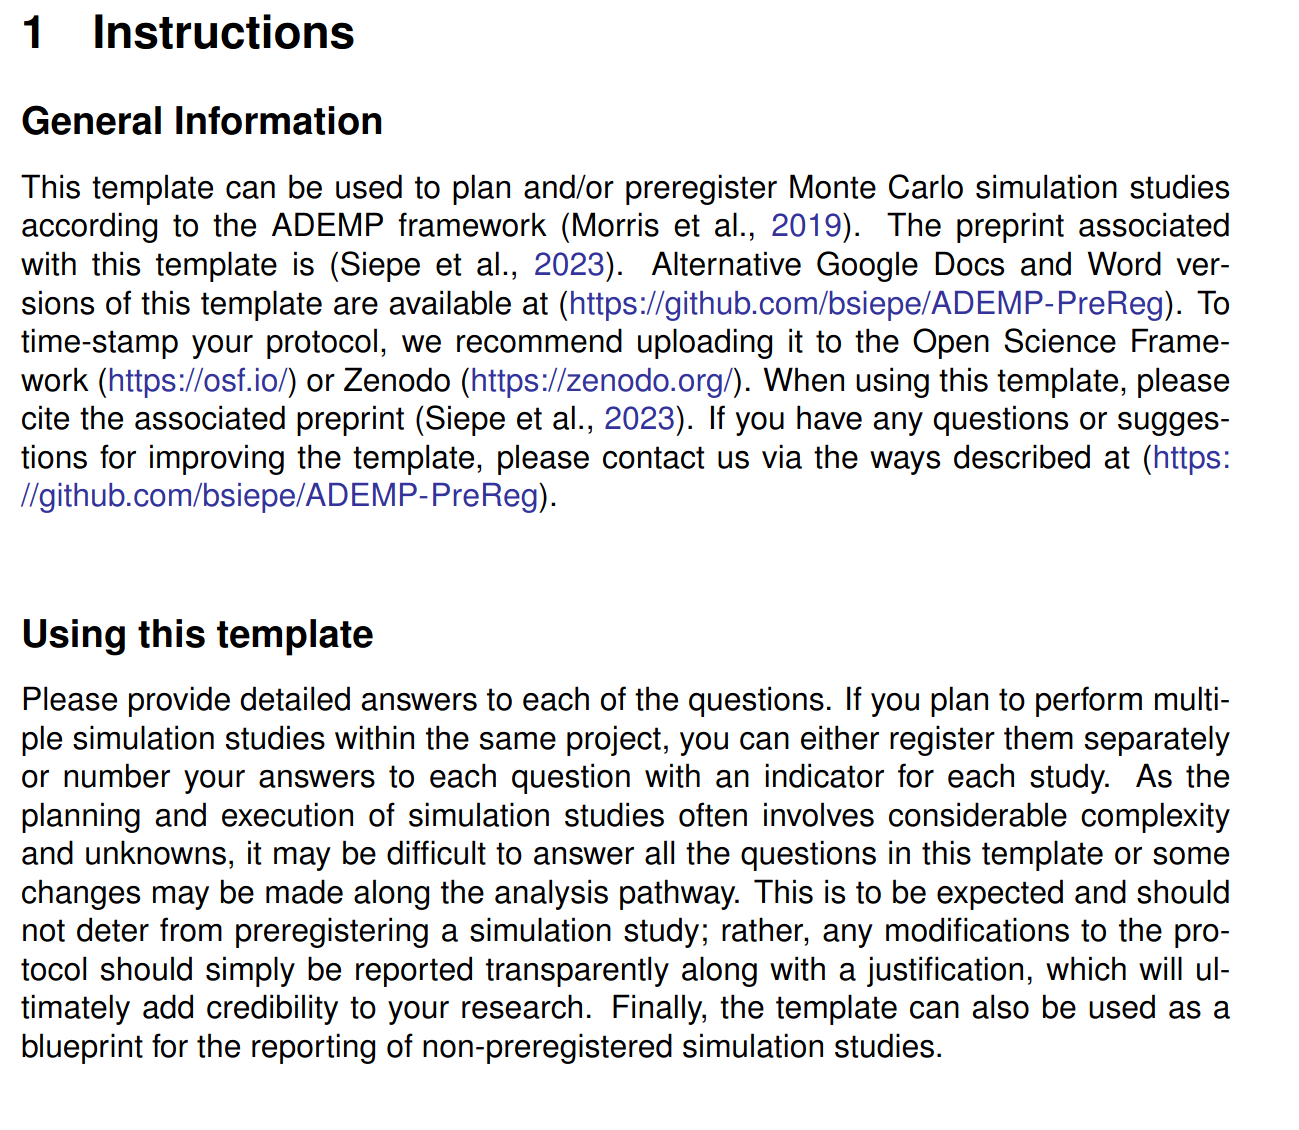
\includegraphics[width=\textwidth,frame]{pics/1instructions.png}}
    % \only<2>{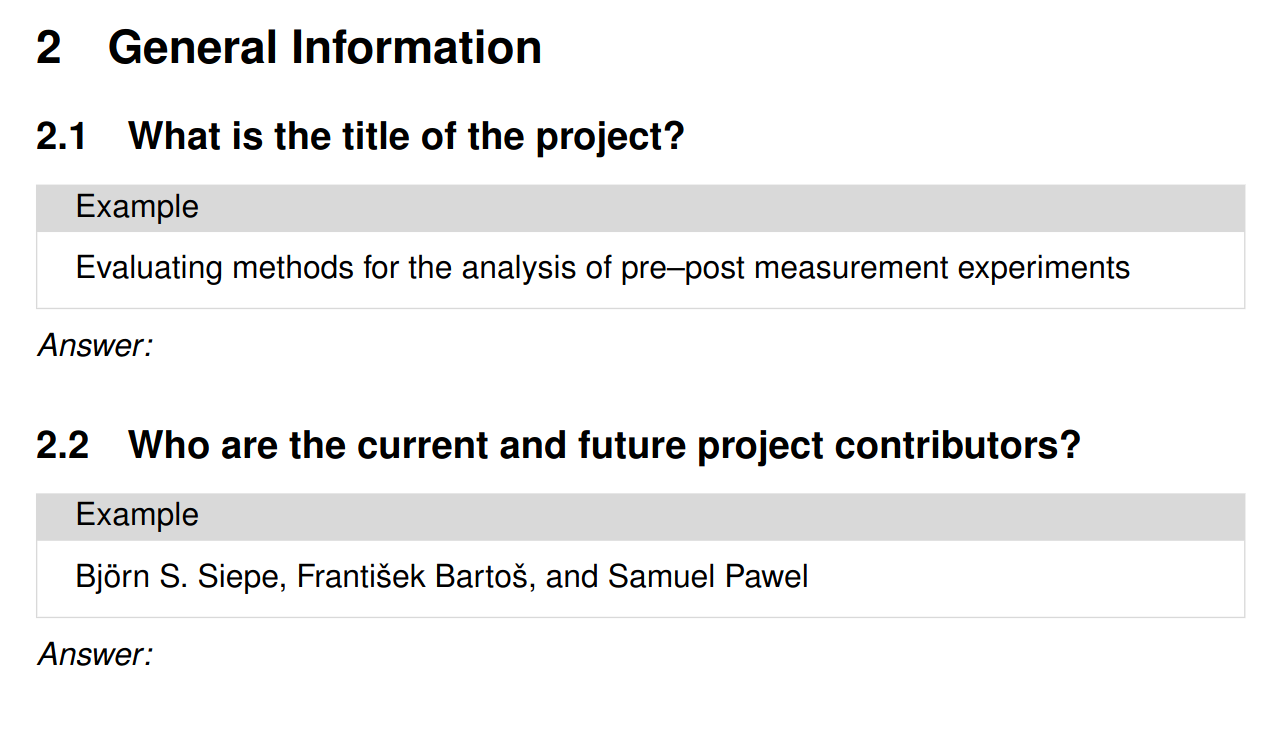
\includegraphics[width=\textwidth,frame]{pics/2general.png}}
    % \only<3>{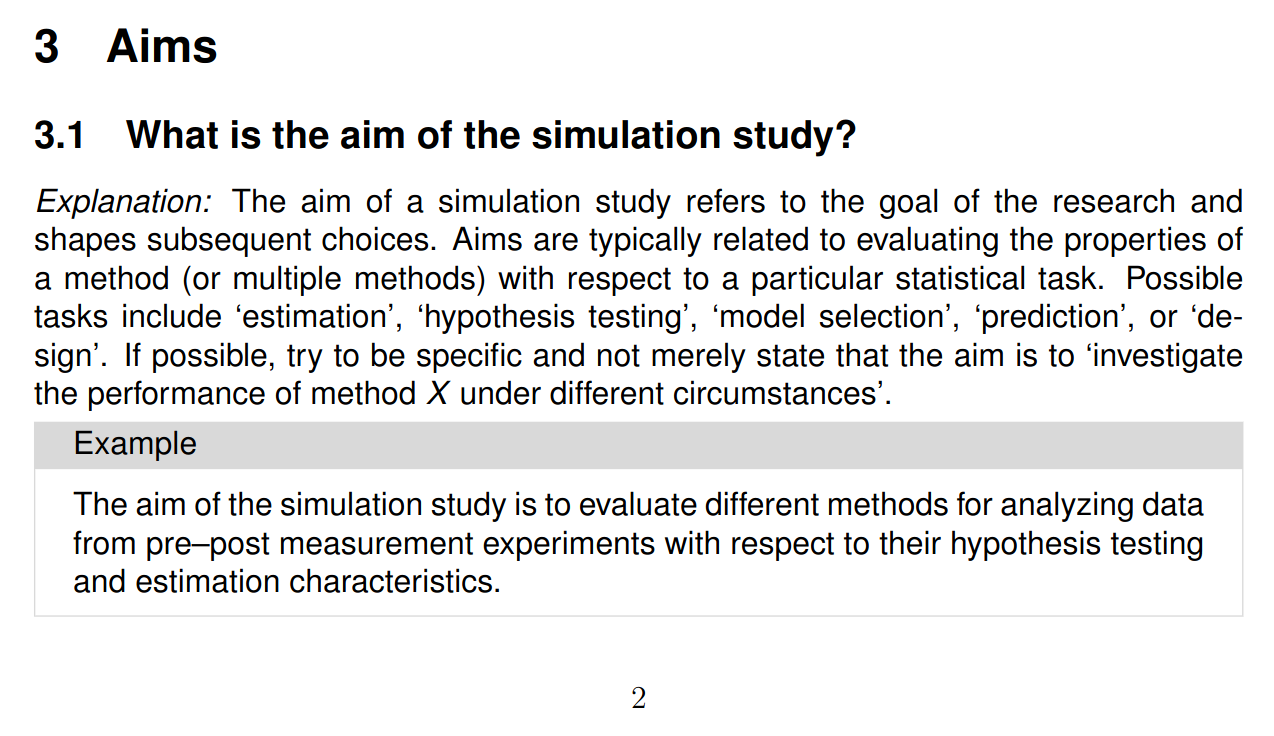
\includegraphics[width=\textwidth,frame]{pics/3aims.png}}
    % \only<4>{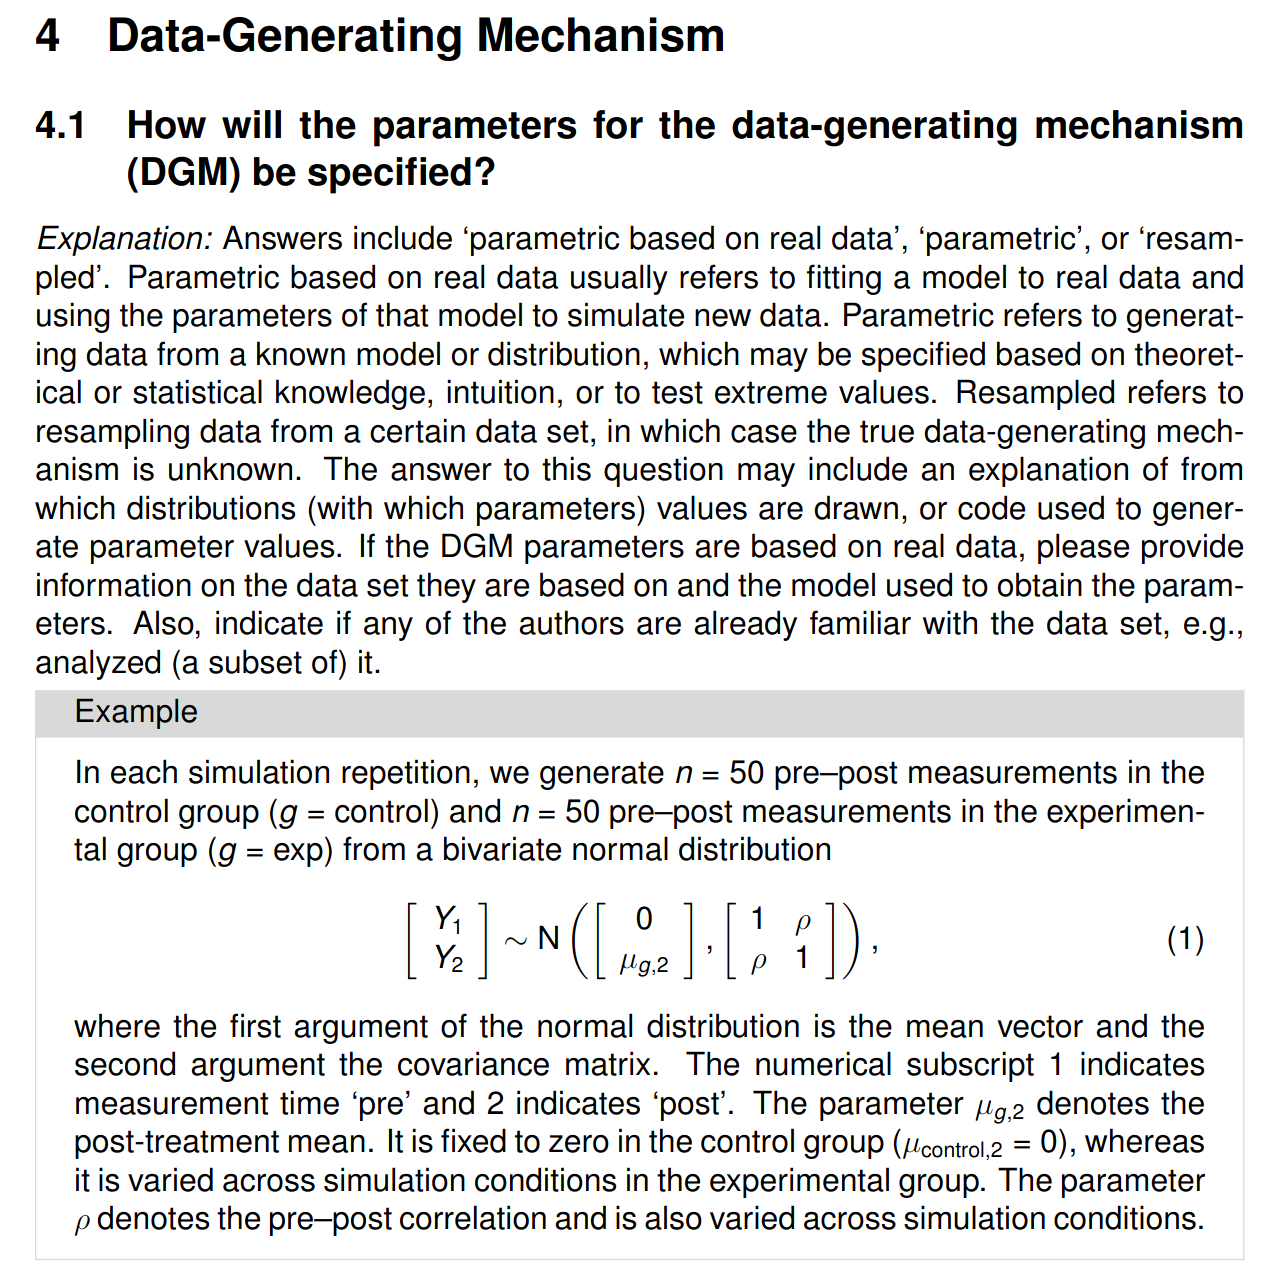
\includegraphics[width=\textwidth,frame]{pics/4dgm.png}}
    % \only<5>{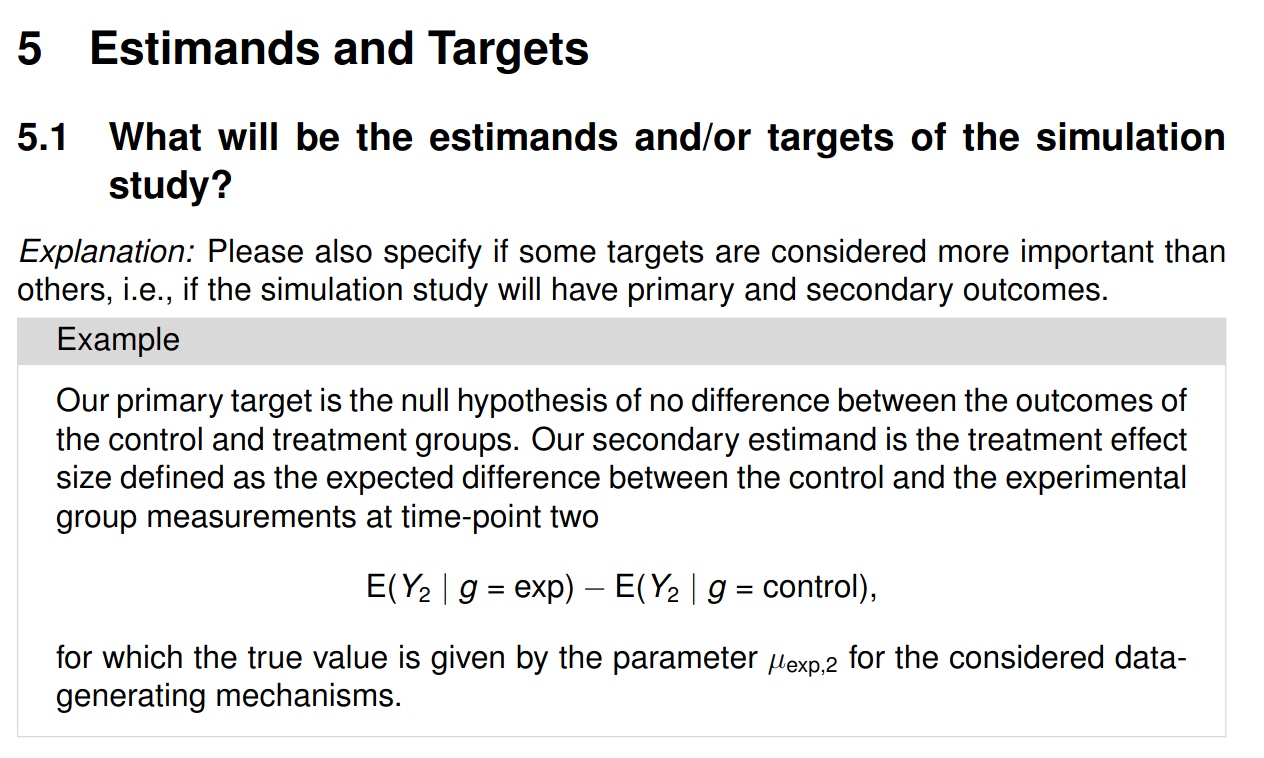
\includegraphics[width=\textwidth,frame]{pics/5estimands.png}}
    % \only<6>{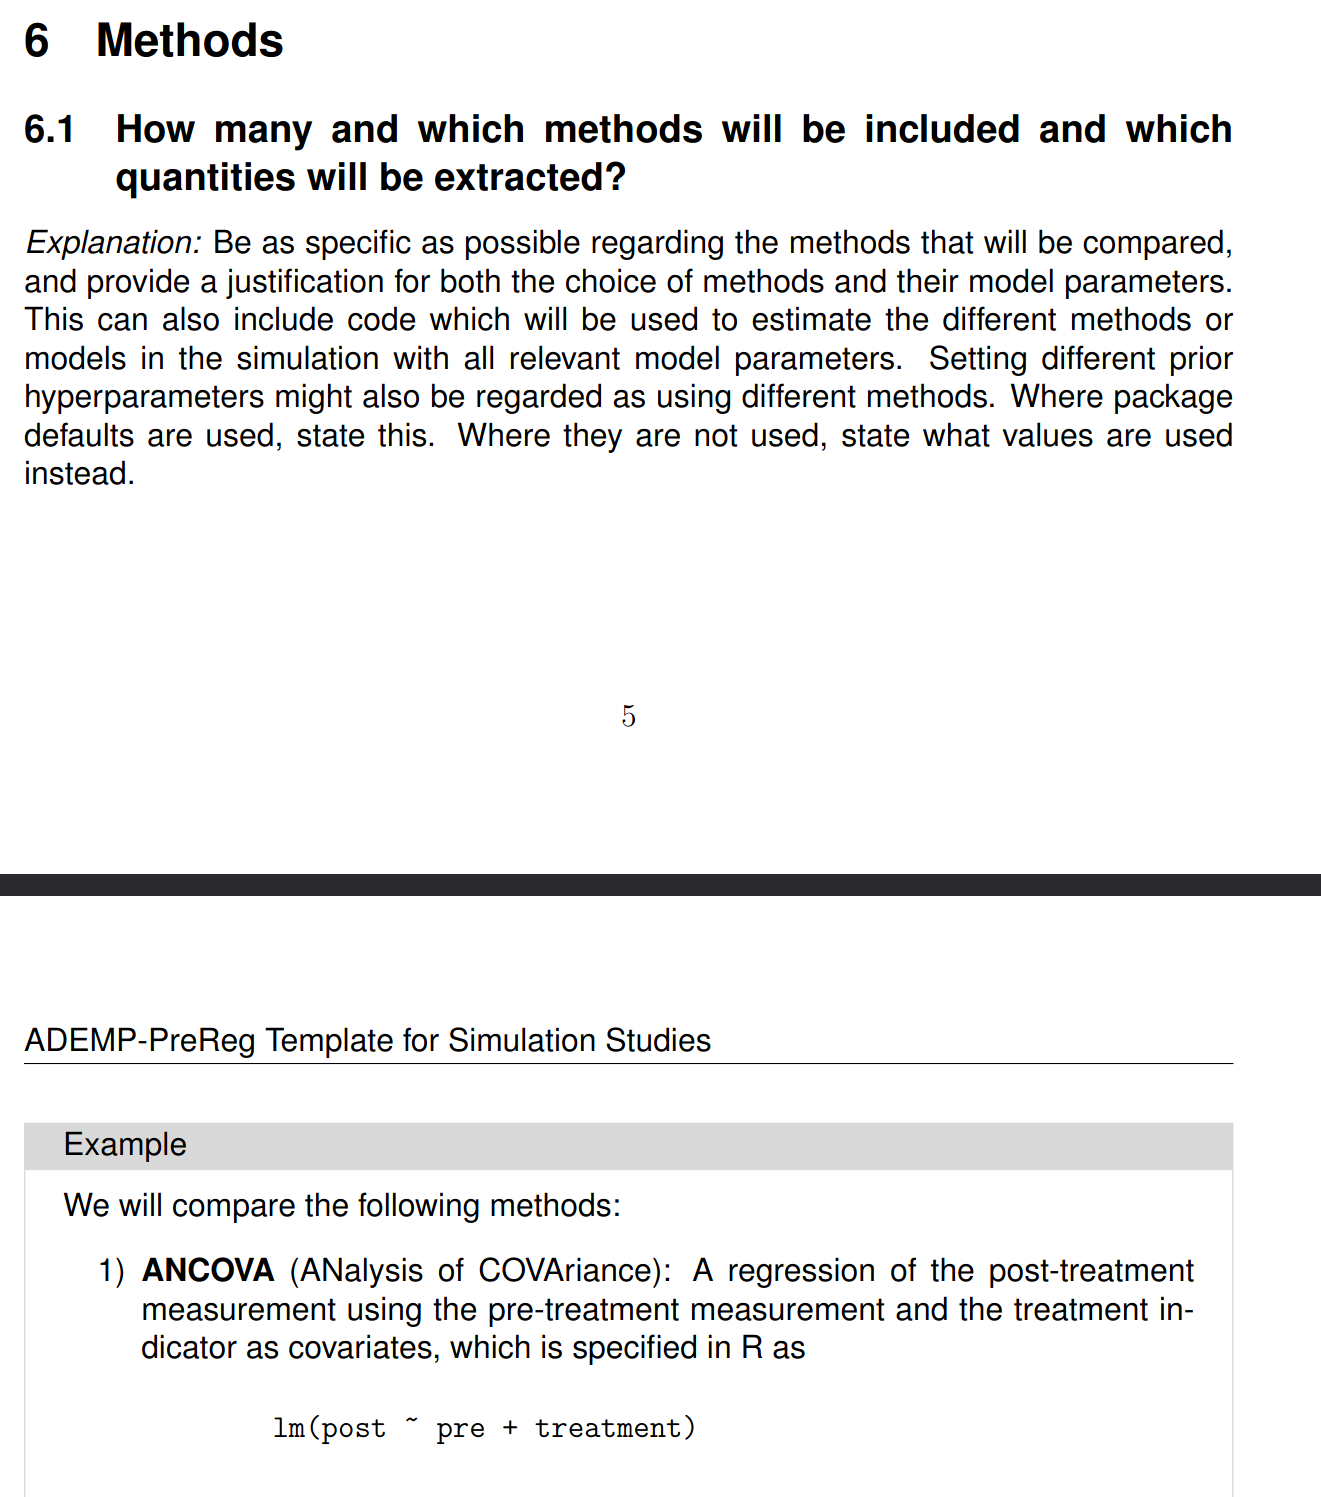
\includegraphics[width=\textwidth,frame]{pics/6methods.png}}
    % \only<7>{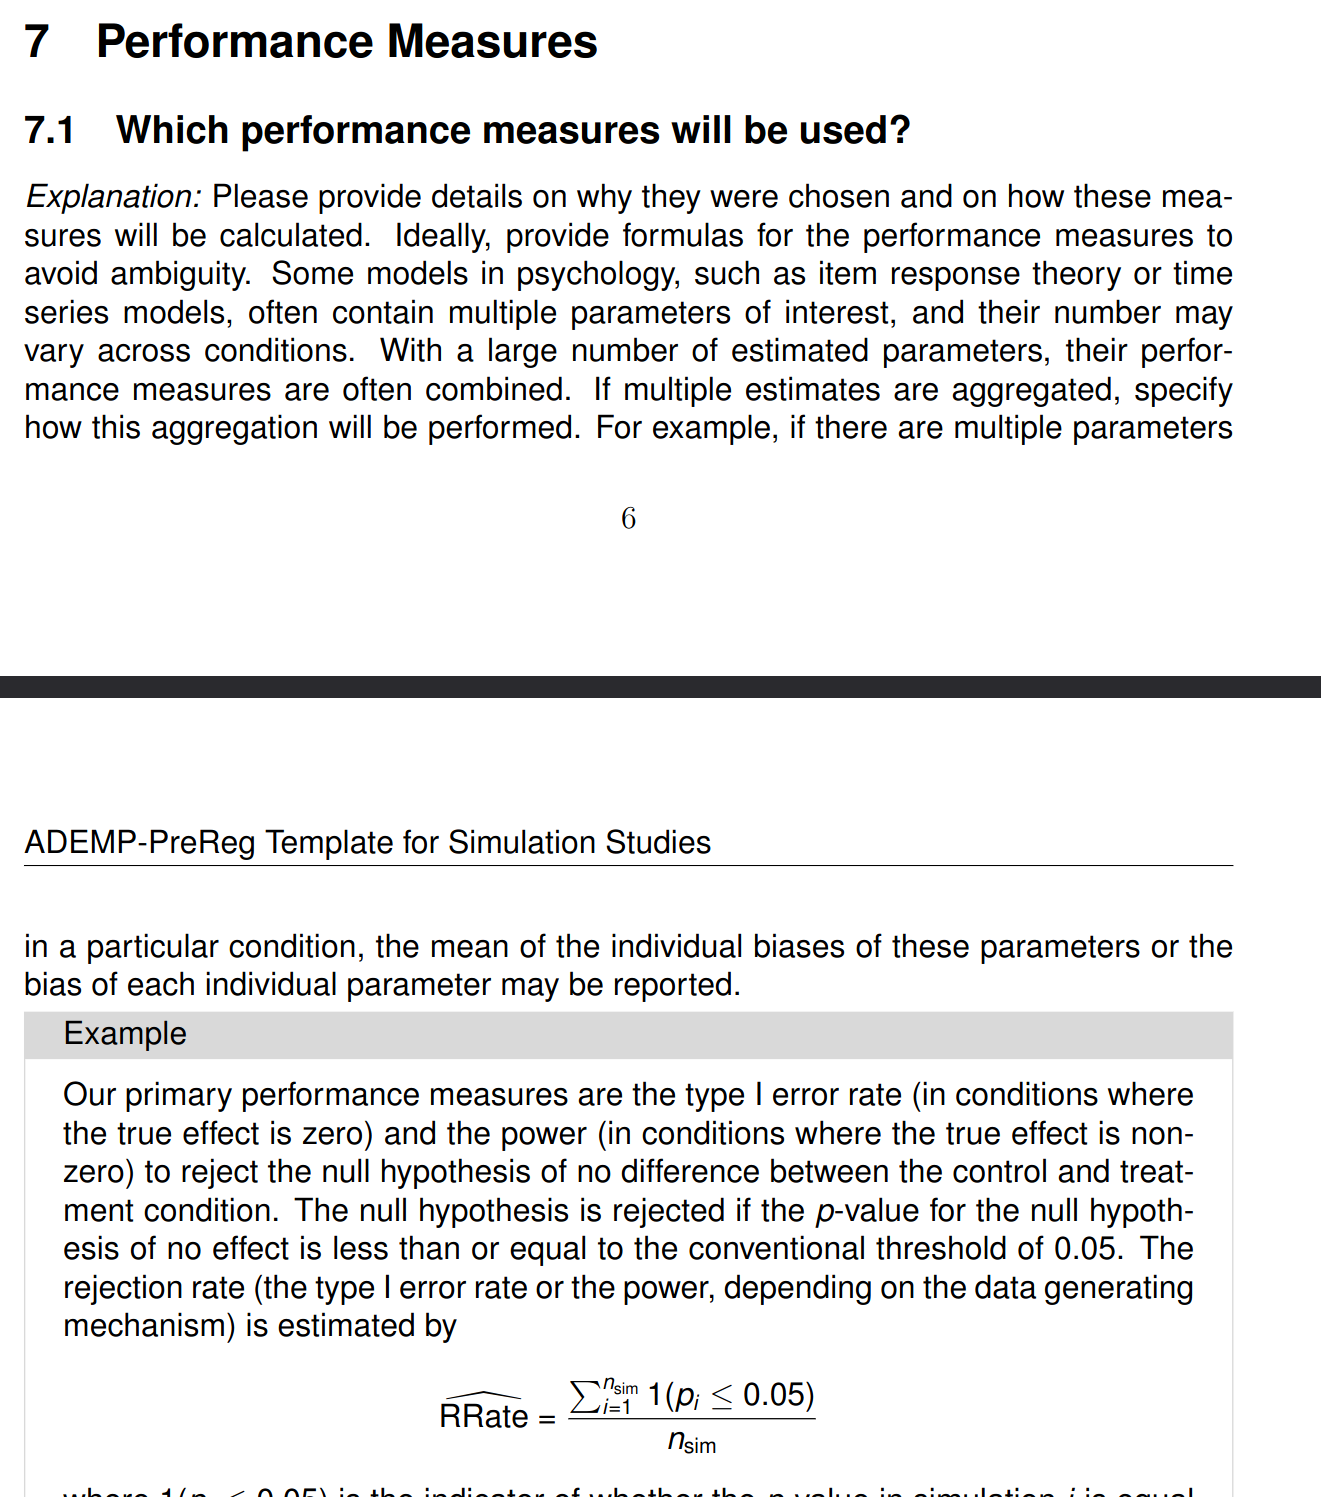
\includegraphics[width=\textwidth,frame]{pics/7performance.png}}
    % \only<8>{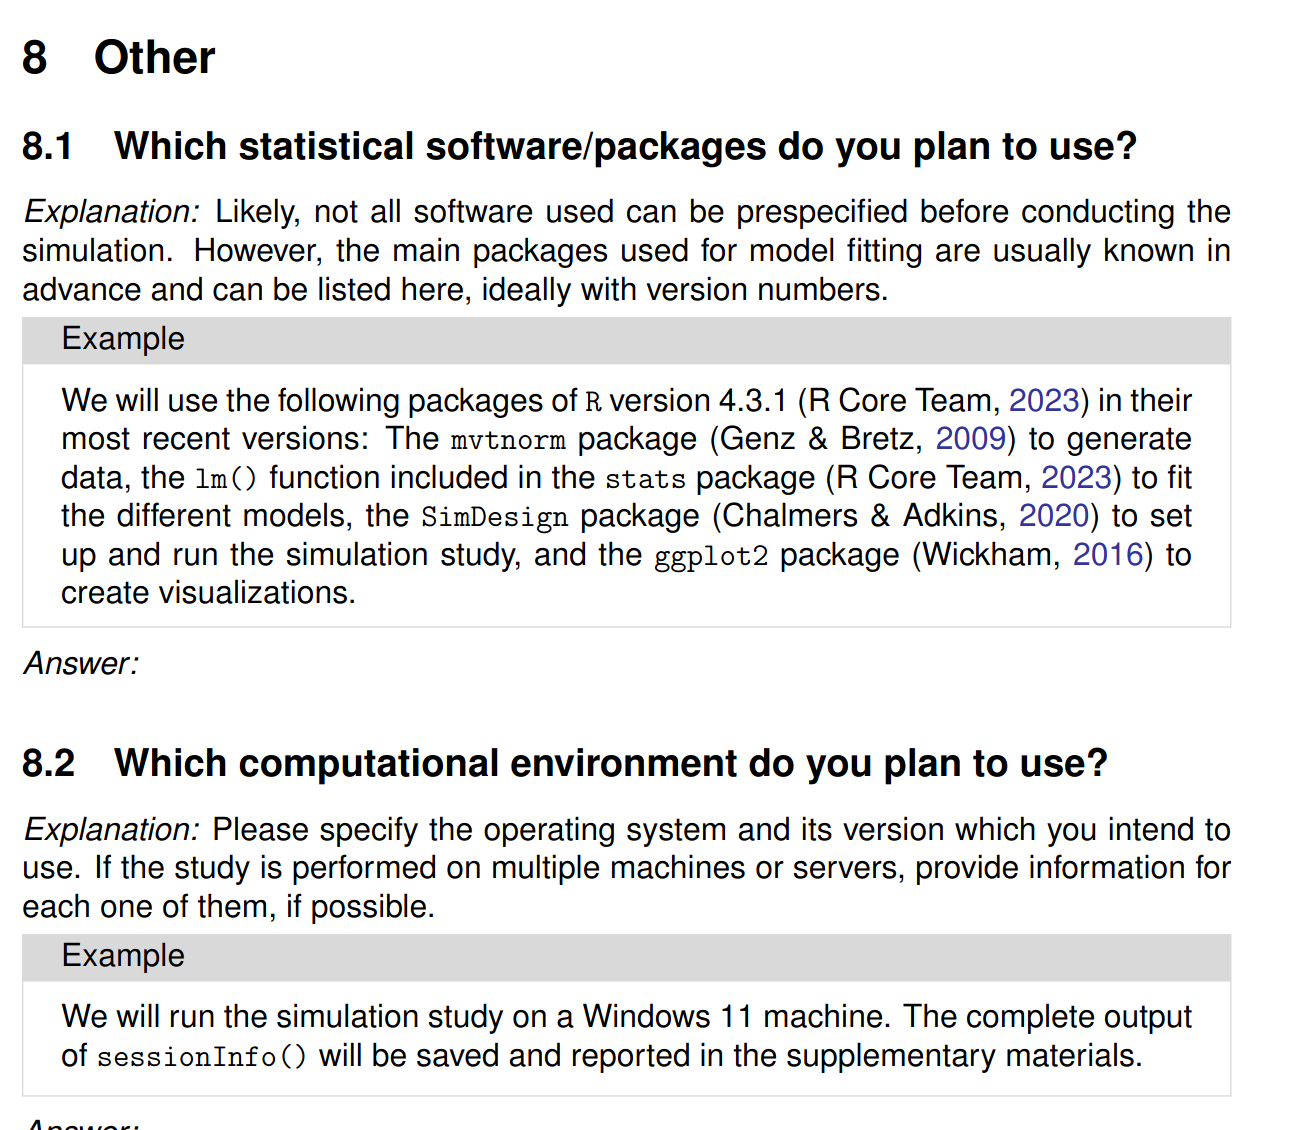
\includegraphics[width=\textwidth,frame]{pics/8other.png}}
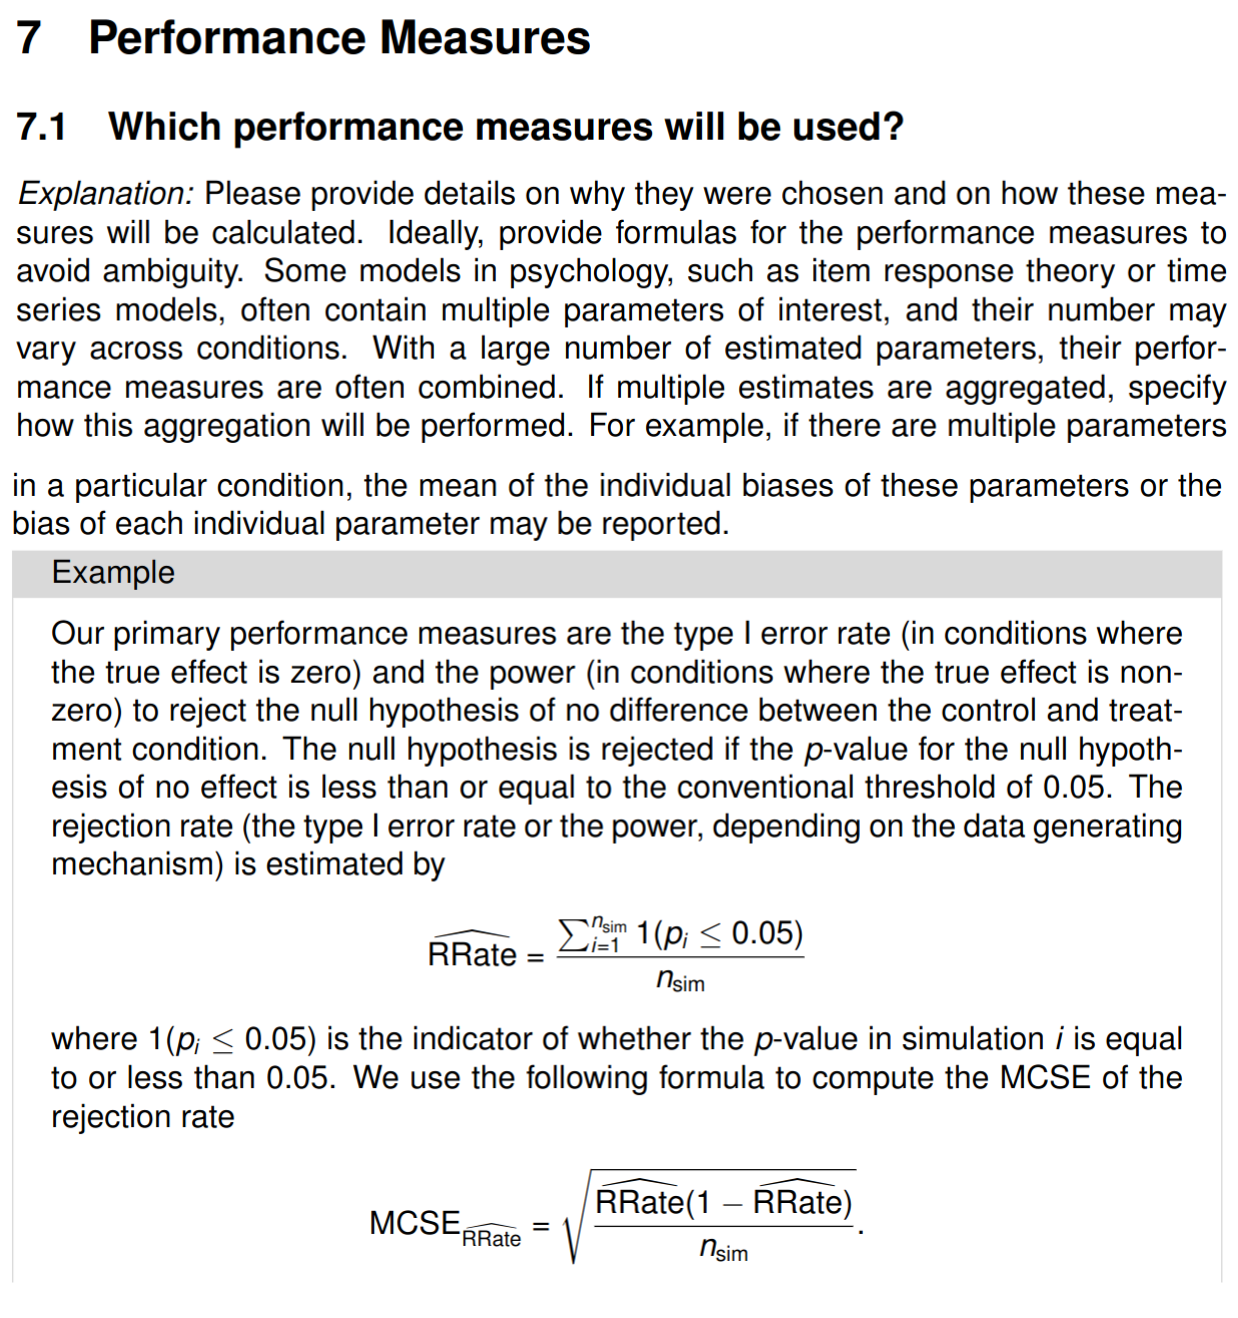
\includegraphics[width=0.9\textwidth,frame]{pics/7performance2.png}
\end{column}
\end{columns}
\end{frame}

\begin{frame}{The ADEMP-PreReg template}
  \begin{columns}
    \begin{column}{0.6\textwidth}

  \begin{block}{Purposes}
    \begin{itemize}
      \pause
      \item \alert{\textbf{Planning}} of simulation studies
      \pause
      \item \alert{\textbf{Preregistration}}
      \pause
      \item Blueprint for \alert{\textbf{reporting}}
      \pause
      \item \alert{\textbf{Reviewing}} of simulation studies
    \end{itemize}
  \end{block}

  \begin{block}{Limitations}
    \begin{itemize}
    \pause
      \item Preregistration could be \alert{\textbf{faked}}
    \pause
      \item May \alert{\textbf{slow down}} exploratory research
    \end{itemize}

  \end{block}
  \end{column}
  \begin{column}{0.4\textwidth}
\centering
    
\includegraphics[width=\textwidth]{pics/CRScycle.JPG} \\
    {\tiny \color{gray} \href{https://zenodo.org/doi/10.5281/zenodo.7994221}{doi:10.5281/zenodo.7994221}}


  \end{column}
\end{columns}
\end{frame}


\begin{frame}{Conclusions}

  \begin{block}{}
    \centering
    
\includegraphics[width = 0.75\textwidth,frame]{pics/siepeetal.png}

    \begin{itemize}
    \pause
      \item Simulation studies can have \alert{\textbf{big impact}}, should be
            \alert{\textbf{conducted carefully}}
      \pause
      \item \alert{\textbf{Protocols}} can make simulation studies
            \alert{\textbf{more reliable}}
      \pause
      \item \alert{\textbf{ADEMP-PreReg template}} helps in preregistration,
            planning, reporting, reviewing of simulation studies
    \end{itemize}
  \end{block}

  {\tiny \color{gray} \href{https://doi.org/10.1037/met0000695}{https://doi.org/10.1037/met0000695}. Slides and manuscript at \href{https://bsiepe.github.io}{https://bsiepe.github.io}.}
\end{frame}

\begin{frame}[allowframebreaks]{References}
\scriptsize
  \bibliographystyle{apalikedoiurl}
  \bibliography{bibliography.bib}
\end{frame}

\end{document}
